\section{Detailed results and mechanism analysis}
\label{sec:extended}
\subsection{Offline behavior at both recorded budgets}
The replay configuration records budgets 320 and 640. Figure~\ref{fig:budgets}
shows both, retaining budget 640 as the primary offline result. Each point
aggregates 20 policy trajectories on the same frozen 16-by-160 correctness and
token matrix. The comparison reuses one observation state for the two survivor
rules at a given budget and seed; unlike the online experiment, there is no
subsequent divergence in candidate generation.

\begin{figure}[tbp]\centering
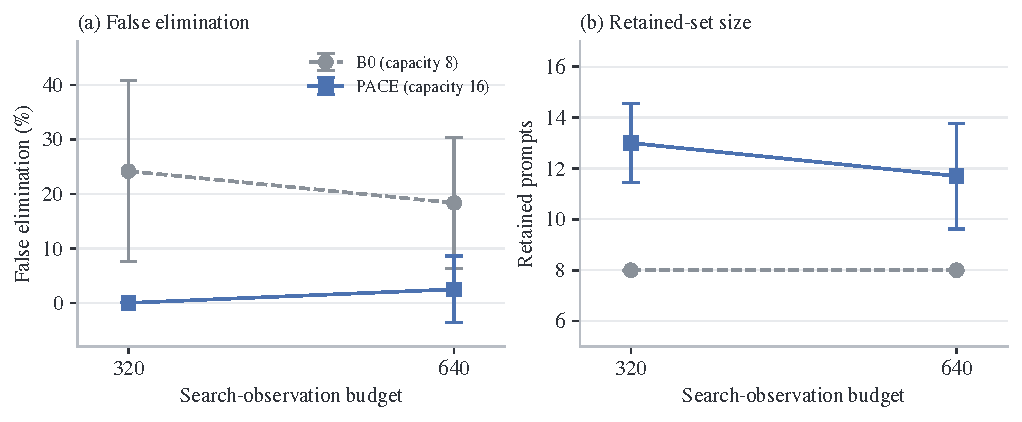
\includegraphics[width=\linewidth]{replay_budgets.pdf}
\caption{Offline replay across the two recorded budgets. Points and error bars
are means and $\pm1$ sample standard deviation across 20 replay seeds. Left:
false-elimination rate. Right: retained-set size. The unequal capacity limits
remain part of the comparison at both budgets; lines only join recorded settings.}
\label{fig:budgets}
\end{figure}

Increasing the observation budget changes the evidence available for the gate
and can alter estimated fronts. It does not remove the retention-capacity
confound: PACE can keep up to all 16 original prompts, whereas archive-free B0
must discard eight. The appropriate interpretation is therefore that the combined
configuration changes finite-pool retention, not that the graph estimates an
isolated causal effect of a calibrated confidence procedure.

The retained-set regret in the offline table is an audit utility gap. An auditor
uses full search-matrix estimates to choose the best retained prompt and compares
it with the best prompt in the complete frozen pool under the same fixed utility.
This differs from the online procedure, where the winner is chosen using partial
search observations and only that winner receives a held-out evaluation. A zero
offline retained-set regret means that at least one utility-optimal reference
candidate remains available; it does not imply that every Pareto candidate was
retained or that a noisy final selector would choose the oracle-preferred one.

\subsection{Search trajectories and capacity pressure}
Figure~\ref{fig:dynamics} summarizes cumulative observation acquisition and
retained-set size at the seven survivor checkpoints. Both methods approach the
same observation cap, yet their candidate counts need not coincide. PACE can
remove a prompt before the set exceeds capacity, while the control only removes
prompts through rank/crowding truncation. Similar total budgets therefore do not
imply identical allocation among candidates or equal information per survivor.

\begin{figure}[tbp]\centering
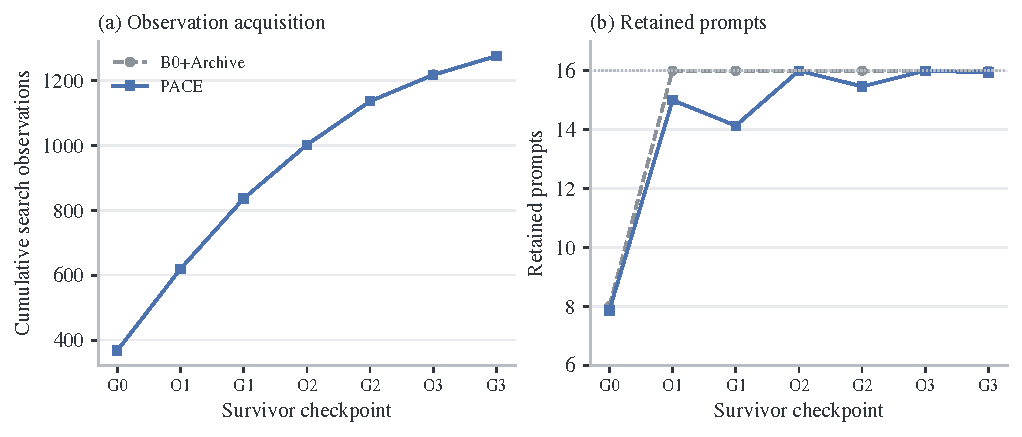
\includegraphics[width=\linewidth]{search_dynamics.pdf}
\caption{Mean online trajectories across 15 paired seeds. Checkpoints alternate
between generation Racing ($G$) and offspring evaluation ($O$); lines show the method means. Left: cumulative acquired search observations.
Right: retained candidate count. Counts are measured after survival; the dashed
line is the matched total capacity of 16. No intermediate test accuracy is implied.}
\label{fig:dynamics}
\end{figure}

The logs allow a description of removal decisions without assigning each removal
a counterfactual value. PACE has 3.80 confidence eliminations and 12.27 forced
evictions per run on average, compared with zero and 16.00 for B0+Archive.
The audit's mean per-run forced-removal share is 0.765 for PACE. This is a mean
of ratios and should not be confused with the ratio of the two mean counts.
The confidence gate relocates some decisions, but forced capacity decisions
still account for most recorded removals.

\begin{table}[tbp]\centering\small
\caption{Descriptive archive audit of the 15 primary paired runs. Search accuracy
is computed on observed search data; it is not an additional held-out score.
Transition rates are proxies derived from active/retained IDs.}
\label{tab:archive}
\begin{tabularx}{\linewidth}{@{}>{\raggedright\arraybackslash}Xrr@{}}\toprule
Signal & B0+Archive & PACE\\\midrule
Confidence eliminations per run & 0.00 & 3.80\\
Forced evictions per run & 16.00 & 12.27\\
Mean within-run forced-removal share & 1.000 & 0.765\\
Never-breeding share of archive-slot steps & 0.436 & 0.465\\
Archive-only IDs later active before offspring & 0.555 & 0.520\\
Mean final archive search accuracy & 0.755 & 0.787\\
Mean final active search accuracy & 0.762 & 0.769\\
Runs whose winner was ever archive-only & --- & 0.200\\\bottomrule
\end{tabularx}
\end{table}

Table~\ref{tab:archive} shows why archive occupancy is not equivalent to productive
protection. Roughly half of archive-only IDs later become active before an
offspring step, but a substantial portion of archive-slot occupancy belongs to
IDs that never do so. The two rates have different denominators: one counts
candidate transitions and the other counts occupied slots over time. They need
not sum to one. Final archive search accuracy is not lower than final active
accuracy for PACE, which also argues against interpreting every unused archive
slot as obviously poor. Selection, sample counts and observation histories all
affect those descriptive averages.

\subsection{Sensitivity to the exploratory cohort and individual seeds}
\label{sec:sensitivity}
The first three paired seeds contribute a mean difference of 4.83 percentage
points, whereas the subsequent 12 contribute 0.92 points. Their weighted mean is
1.70 points. Figure~\ref{fig:sensitivity} makes this decomposition visible and
shows leave-one-seed-out means. These are post-hoc descriptions of the existing
runs, not new confirmatory experiments or alternative primary analyses.

\begin{figure}[tbp]\centering
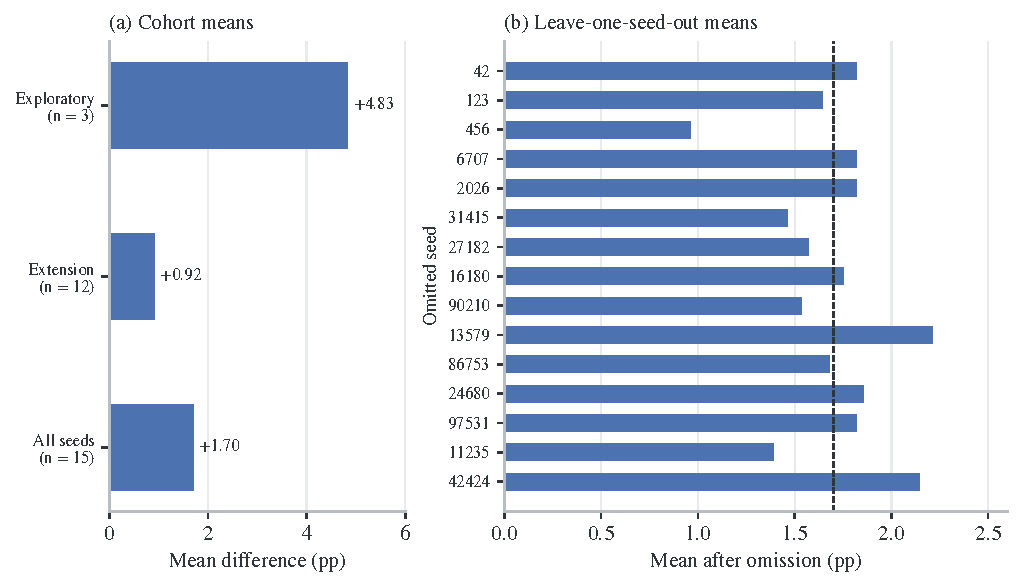
\includegraphics[width=\linewidth]{seed_sensitivity.pdf}
\caption{Descriptive sensitivity analysis. Left: cohort means and sample sizes,
with no inferential error bars. Right: means after omitting each paired seed in
turn, in protocol order. The dashed reference is the full 15-seed mean. Omission
is diagnostic only; no seed is excluded from the primary analysis.}
\label{fig:sensitivity}
\end{figure}

The largest individual gain is 12.0 percentage points at seed 456, and the largest
loss is 5.5 points at seed 13579. Omitting one seed at a time yields means from
0.96 to 2.21 points. This is the range of omission means, not a confidence interval. A positive mean throughout these omissions does
not overturn the primary interval crossing zero. The extension-only mean is
likewise not independent replication across tasks: it uses the same fixed model,
manifest, operators and held-out examples.

\subsection{Contrasting winner examples}
For seed 456, the control winner achieves 65.5\% and the PACE winner 77.5\%.
The control text contains an abbreviated definition header, while the PACE text
combines a librarian role with an explicit single-label instruction. For seed
13579, the control achieves 82.0\% and PACE 76.5\%, with the control using a
longer canonical-label format instruction. Exact strings appear in
Appendix~\ref{app:prompts}. These cases show that the same operator family can
produce both gains and losses; they do not establish a general rule that roles,
length, or a particular wording cause better classification.

Seed 42 is a useful contrast: both searches select exactly the same instruction
string and reach 85.5\% accuracy, even though generated IDs carry different method
prefixes. An unchanged winner can coexist with different survival logs. Changes in the survivor logs can therefore occur without changing the
selected instruction. The winner-only evaluation protocol supports these endpoint
comparisons, but does not provide class-level explanations, per-example paired
error tests, or a held-out trajectory for every generated candidate.
